\chapter{Implémentation}

% Containing a comprehensive description of the implementation of your software, including the language(s) and platform chosen, problems encountered, any changes made to the design as a result of the implementation, etc.
Ce chapitre donne quelques éclaircissements quant à l'architecture soit globale soit celle de l'application mobile tout en mettant le doigt sur les problèmes rencontrés, ensuite il liste les différentes technologies utilisées, enfin il justifie nos choix techniques.
\section{Architecture} % (fold)
\label{sec:architecture}
\subsection{Architecture globale} % (fold)
\label{ssub:architecture_globale}
L’architecture globale de mise en œuvre est illustrée par la figure \Figref{architecture.png}. Cette architecture est subdivisée en 3 couches et repose sur l’utilisation des services Web, qui ont pour objectif d’assurer une flexibilité d’échange de services entre les différents composants du système.\newline
Les différentes parties vont être décrits comme suit :
\begin{enumerate}
	\item Couche présentation : c'est notre application cliente dans notre cas mobile, qui tourne sur le système IOS ou Android et assure l'affichage et le dialogue avec l'utilisateur.
	\item Coté serveur : assure le traitement métier des données et correspond à la mise en œuvre de l'ensemble des règles de gestion et de la logique applicative, cette partie contient deux principaux services Web : l'un gère les covoiturages instantané et l'autre planifié. Elle est hébergée sur le cloud Digital Ocean :
	\begin{itemize}
		\item Service de covoiturage instantané : il assure les demandes et offres de covoiturage temps réel en utilisant l'algorithme de matching. chaque fois qu'un passager lance une offre il est intercepté par ce service qui lance le processus du matching. 
		\item Service de covoiturage planifié : il est responsable des demandes et offres de covoiturage planifié ou statique. il est sollicité chaque fois une offre ajouté ou à chaque demande de prise en charge d'un passager par un conducteur.
	\end{itemize}
	Nos API ou services sont conformes au standard REST (representational state transfer), donc la communication entre ses services est basée sur le protocole Http. Outre ils respectent des contraintes architecturales comme : La communication client–serveur s'effectue sans conservation de l'état de la session de communication sur le serveur entre deux requêtes successives.\cite{fielding2000architectural}
	\item Base de données : Elle correspond à la partie gérant l'accès aux données de l'application, deux bases de données sont utilisées :
	\begin{itemize}
		\item MySql : les informations sur les utilisateurs, les offres planifiés où autres donnés qui ne changent pas souvent, résident sur cette base.
		\item Firebase : les données comme les offres instantanée et les positions des conducteurs sont sollicités en lecture en temps réel, donc ils seront hébergés sur cette base.
	\end{itemize}
\end{enumerate}
\fig{architecture.png}{architecture de l'application}{0.5}
% subsubsection architecture_globale (end)
\subsection{Architecture client side}
\subsubsection{MVC} % (fold)
 \label{ssub:mvc}
 Commençons par définir ce que c'est que MVC. Le Model View Controller permet de diviser son programme en trois parties indépendantes :
 \begin{itemize}
 	\item Le modèle : il contient la logique de l'application, il renferme nos entités qui sont des classes ou structures qui interagissent entre eux, et aussi les servies qui peuvent par exemple faire des appels réseau ou accéder à une base de données.
 	\item Le contrôleur : il récupère  et formate les informations du modèle pour les passer à la vue.
 	\item La vue : c'est ce que l'utilisateur voit, c'est l'interface de l'application.
 \end{itemize}
 Apple a choisi par défaut le très populaire patron de conception architectural MVC pour les applications iPhone\cite{mvc}. Cela veut dire que la façon dont ils ont conçu le développement d'application iPhone nous encourage à respecter ce design. \newline
 MVC avant tout, est un ensemble de règles de communication :
 \begin{itemize}
 	\item La vue et le modèle ne peuvent \textbf{JAMAIS} communiquer. chacun d'eux ignore l’existence de l'autre.
 	\item Le modèle peut parler indirectement au contrôleur par des notifications ou des fermetures (closures). C'est une communication aveugle, c'est à dire le modèle ne contient pas de référence du contrôleur.
 	\item La vue parle au contrôleur en lui délégant la gestion des interactions de l'utilisateur avec l'application, le contrôleur dans ce cas s'engage à répondre à sa demande comme montre la figure 
 	\fig{target_action.jpg}{le patron de conception target-action}{0.4}\newline
 \end{itemize}
 La figure\Figref{mvc.png} résume ce qui a été dit dans cette partie.
 \fig{mvc.png}{patron de conception mvc}{0.2}
 % subsubsection mvc (end) 

 \subsubsection{Difficultés rencontrées} % (fold)
 \label{ssub:difficultés_rencontrées_et_pourquoi_mvvm_}
 Au fur et à mesure que notre application croît en taille et en portée, les problèmes complexes de maintenance commencent à surgir. Nous avons rencontré beaucoup de difficultés à tester nos contrôleurs et ce, même en essayant de les alléger et de déléguer beaucoup de fonctionnalités à des classes de services ou modèle. C'est ce qui nous a poussé à adopter une nouvelle structuration du code : le modèle MVVM.\cite{mvvm}\newline
 MVVM vise à exporter les traitements de la logique de présentation dans des entités à part entière qui s'appellent les ViewModels, et qui seront placées entre la Vue/Contrôleur (qui désormais constitue une seule entité) et le modèle comme montre la figure\Figref{mvvm.png}.
 \begin{itemize}
 	\item Le modèle : reste le même que celui de MVC.
 	\item La vue/contrôleur : cette couche représente le contexte de l'interface utilisateur et ses interactions. Désormais, nous considérons les vues et leurs contrôleurs MVC comme une seule entité.
 	\item Le View Model : le rôle qui incombe au ViewModel est de récupérer les données à partir du modèle et de les rendre disponibles à la vue sous une meilleure forme. De cette manière, on aura des contrôleurs beaucoup moins chargées qu'avant. On aurait allégé les tests UI puisqu'on a transformé une grande partie des contrôleurs en un modèle de données testable unitairement.
 \end{itemize}
 \fig{mvvm.png}{le patron de conception MVVM}{0.2}
 Puisque je me suis penché plus sur le développement de l'application partie cliente sur ios, je vais me limiter à décrire les outils utilisés dans cette partie par la suite.
 % subsubsection difficultés_rencontrées_et_pourquoi_mvvm_ (end)
% section architecture (end)

\section{Technologies utilisées} % (fold)
\label{sec:technologies_et_outils_utilisés}
\subsubsection{Langages} % (fold)
\label{ssub:lanages}
\begin{itemize}
	\itemb \textbf{Objective-C} : C'est une extension du C ANSI, comme le C++, mais qui se distingue de ce dernier par sa distribution dynamique des messages, son typage faible ou fort, son typage dynamique et son chargement dynamique. il est principalement utilisé dans les systèmes d'exploitation d'Apple.
	\itemb \textbf{Swift} : un langage de programmation objet compilé, multi-paradigmes, ayant pour objectif d'être simple, hautes performances et sûr. Il est développé en open source.
\end{itemize}
% subsubsection lanages (end)

\subsubsection{Frameworks} % (fold)
\label{ssub:subsubsection_name}
\begin{itemize}
	\itemb \textbf{Cocoa Touch} : il fournit l'infrastructure requise pour les applications iOS ou tvOS. Il fournit l'architecture de fenêtre et de vue pour implémenter l'interface, l'infrastructure de gestion des événements pour fournir Multi-Touch et d'autres types d'entrée à l'application.
	il regroupe deux autres frameworks qui sont Foundation c'est la base comme son nom l'indique, et UIKit
	qui permet de créer des interfaces graphiques.
	\itemb \textbf{Core Data} : c'est un framework qui permet de faire persister les données en local (sur l'iphone), il fournit l’accès a une base de donnée standard (souvent SQLite) et une API orientée objet c'est à dire un ORM (Object Relational Mapping).
	\itemb \textbf{Here} : il permet aux applications clientes d'utiliser les données de cartographie comme colonne vertébrale pour leurs applications mobiles, et aussi d'accéder à des informations telles que les vitesses moyennes sur route, l'accroissement du trafic et les charges maximales pouvant être transportées sur une route particulière
	\itemb \textbf{Firebase} : un BaaS (Back-as-a-a-Service) qui permettra de stocker et de synchroniser les données sur tous vos clients en temps réel. Chaque fois que les données changent, Firebase met à jour les applications sur chaque appareil (mobile ou Web). Si votre application Firebase fonctionne hors ligne, ses données seront synchronisées une fois la connectivité rétablie.\newline
	le SDK pour (Software Developement Kit) de Firebase regroupe tous les API et il est facile a intégrer dans l'application.
\end{itemize}
% subsubsection subsubsection_name (end)

\subsubsection{Outils} % (fold)
\label{ssub:outils}
\begin{itemize}
	\itemb \textbf{Xcode} : un environnement de développement (IDE) pour macOS, Fournit toute une suite logicielle (graphiques, audio, etc.) pour développeurs et programmeurs. Il permet de créer des logiciels pour iOS, watchOS et tvOS.
	\itemb \textbf{CocoaPods} : un gestionnaire de dépendances au niveau de l'application pour Objective-C, Swift et toutes les autres langues qui s'exécutent sur l'environnement d'exécution Objective-C, comme RubyMotion, et qui fournit un format standard pour la gestion des bibliothèques externes. il permet d'automatiser l’intégration des autres frameworks dans un projet.
	\itemb \textbf{Postman} : un outil qui permet d'interroger et tester les webservices et API, il propose de nombreuses fonctionnalités, une prise en main rapide et une interface graphique agréable.
\end{itemize}
% subsubsection outils (end)
% section technologies_et_outils_utilisés (end)

\section{Justification des choix techniques} % (fold)
\label{sec:justification_du_choix_technique}
\subsection{partie cliente} % (fold)
\label{sub:partie_cliente}
\subsubsection{Applications natives} % (fold)
\label{ssub:application_native}
\begin{itemize}
	\item Notre application a besoin d’accéder rapidement à toutes les fonctionnalités du téléphone, du gps en passant par la caméra et le micro.
	\item Les notifications push, uniquement disponibles sur les apps natives occupent une place centrale dans notre app. ils permettent d’alerter les passagers sur l'état de leurs offres ainsi que la position du conducteur en cas de prise en charge. Et au conducteur de recevoir des demandes.
	\item le budget dédié au développement couvre les charges de ces dernières.
\end{itemize}
% subsubsection application_native (end)

\subsubsection{Here} % (fold)
\label{ssub:here}
Dans ce cas le choix sur le prix que propose différents fournisseurs de service de cartographie.\newline
Google a augmenté ses prix de 1400\%. et a limité sa version gratuite. C'est pourquoi ICI (Here) est beaucoup plus attrayant que Google, car nous pouvons utiliser le modèle fremium et utiliser 250 000 appels API par jour. Versus 28.000 de Google.\newline
La figure ci-dessous compare les deux fournisseurs en termes de prix.\cite{heremaps}
\fig{here.png}{HERE Maps API vs Google Maps API}{0.5}
% subsubsection here (end)
% subsection partie_cliente (end)

\subsection{Partie serveur} % (fold)
\label{sub:partie_serveur}

\subsubsection{API Rest} % (fold)
\label{ssub:api_rest}
Comme il a été dit dans la partie spécification des besoins notre application devrait être portable et extensible. les services web REST permet au mieux de répondre à ses exigences et sont plus faciles à implémenter, comparés aux méthodes du type RPC Remote Procedure Call comme SOAP.
% subsubsection api_rest (end)
\subsubsection{Digital Ocean} % (fold)
\label{ssub:digital_ocean}
Puisque notre utilisation du cloud se limite à louer une capacité de calcul et donc pas aux service. on a besoin d'un fournisseur cloud qui gère le matériel serveur, les couches de virtualisation, le stockage, les réseaux)\newline
Digital Ocean  présente une solution qui répond bien à notre besoin d'héberger notre application à moindre coût.\cite{digitalocean}
\fig{digitalocean.png}{Performances CPU par dollar de toutes les machines virtuelles testées}{0.5}
% subsubsection digital_ocean (end)
% subsection partie_serveur (end)

\subsection{Choix du système de gestion de données} % (fold)
\label{sub:partie_base_de_données}
\subsubsection{Mysql} % (fold)
\label{ssub:le_choix_de_mysql}
\begin{itemize}
	\item Le projet MySQL a rendu son code source disponible sous les termes de la GNU General Public License, donc il représente une solution a moindre coût, l'autre avantage est qu'il y a une grande communauté derrière, par conséquent, nous pouvons facilement apprendre et dépanner MySQL à partir de différentes sources comme des blogs, des livres blancs et des livres.
	\item Nous avons pas de données sur le nombre d'utilisateur à venir, donc la mise à l'échelle et la réplication sont des fonctions primordiales et notre SGBD les prennent  en charge.
	\item Les transactions sont simples, les données sur le covoiturage planifié sont le plus souvent demandées en lecture, donc les performances de mysql sont largement suffisantes.
\end{itemize}
% subsubsection le_choix_de_mysql (end)

\subsubsection{Firebase} % (fold)
\label{ssub:firebase}
\begin{itemize}
	\item Dans le cas des données sur le covoiturage dynamique (offres, demandes, position des conducteurs...), l’écriture et la lecture en temps réel est le premier facteur à prendre en compte. la raison derrière le choix est que Firebase est essentiellement un service cloud fourni par Google, il fonctionne donc mieux que les autres serveurs et fournisseurs de services backend. (une étude détaillée nous manquait)
	\item Vu la contrainte temporelle: 4 mois pour développer l'application. Firebase économise beaucoup de temps puisque il offre un ensemble de services prêts à l'emploi, cela veut dire qu'il n'est pas seulement un système de gestion de données mais un logiciel en tant que service SaaS.
	\item En mode développement la plateforme est gratuite.
	\item Firebase c'est tout un eco-systeme donc nous pouvons intégrer gratuitement des services comme Google Analytics qui nous aide à comprendre comment les gens utilisent notre application. L'outil capture automatiquement un certain nombre d'événements et de propriétés utilisateur et permet également de définir nos propres événements personnalisés pour mesurer les éléments qui importent à l'entreprise. 
\end{itemize}
% subsubsection firebase (end)
% subsection partie_base_de_données (end)
% section justification_du_choix_technique (end)
\section{Quelques interfaces utilisateur}
Cette section présente quelques interfaces utilisateur.
\begin{figure}%
    \centering
    \subfloat[L’accueil]{{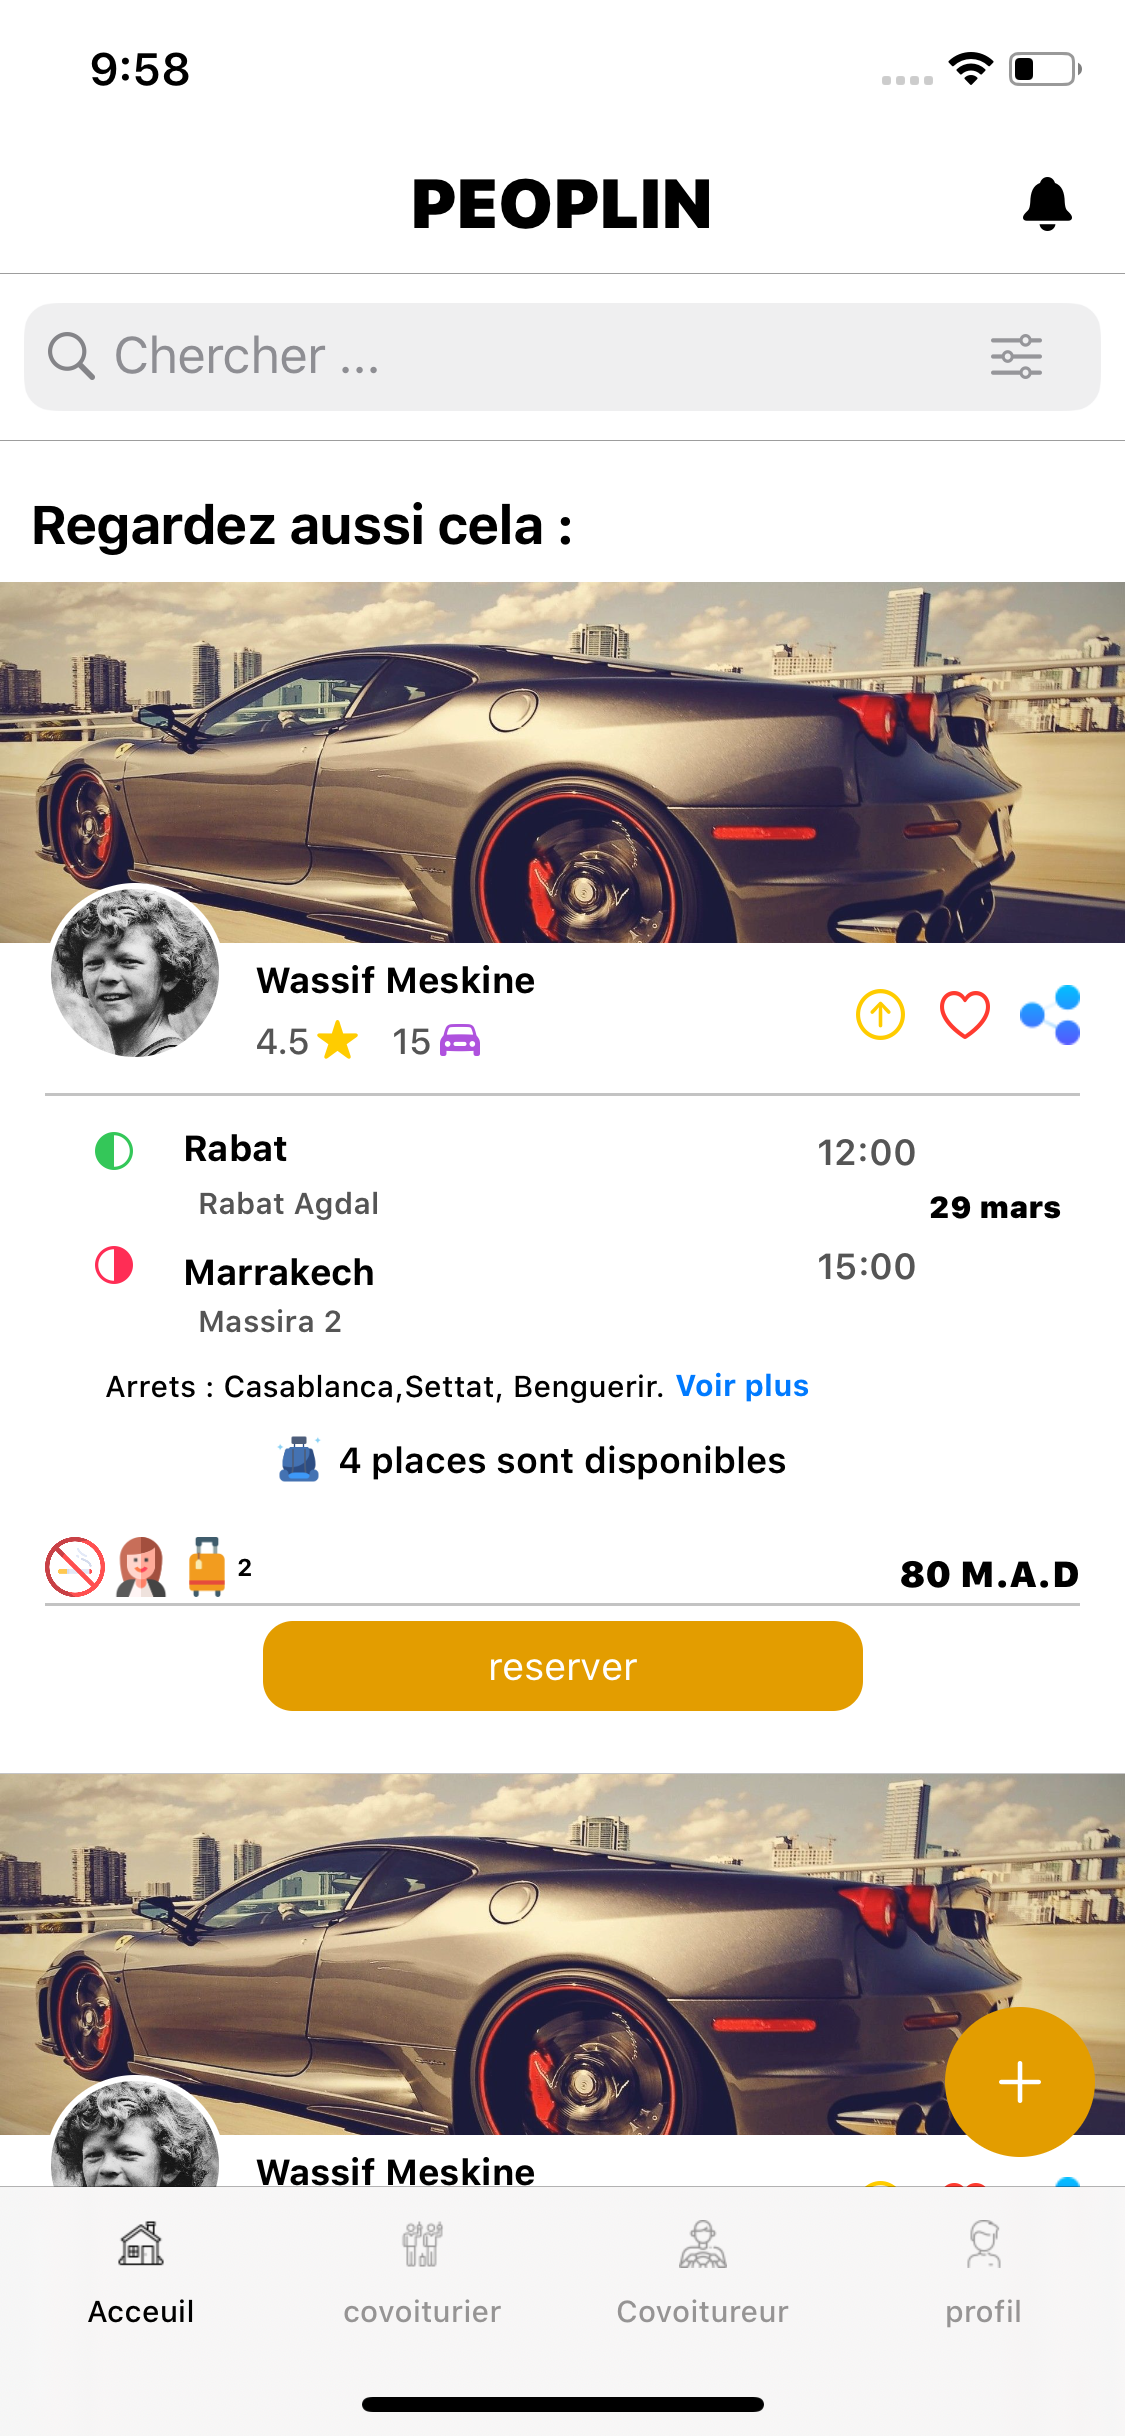
\includegraphics[width=7cm]{figs/ui1.png} }}%
    \qquad
    \subfloat[Ajouter offre planifiée]{{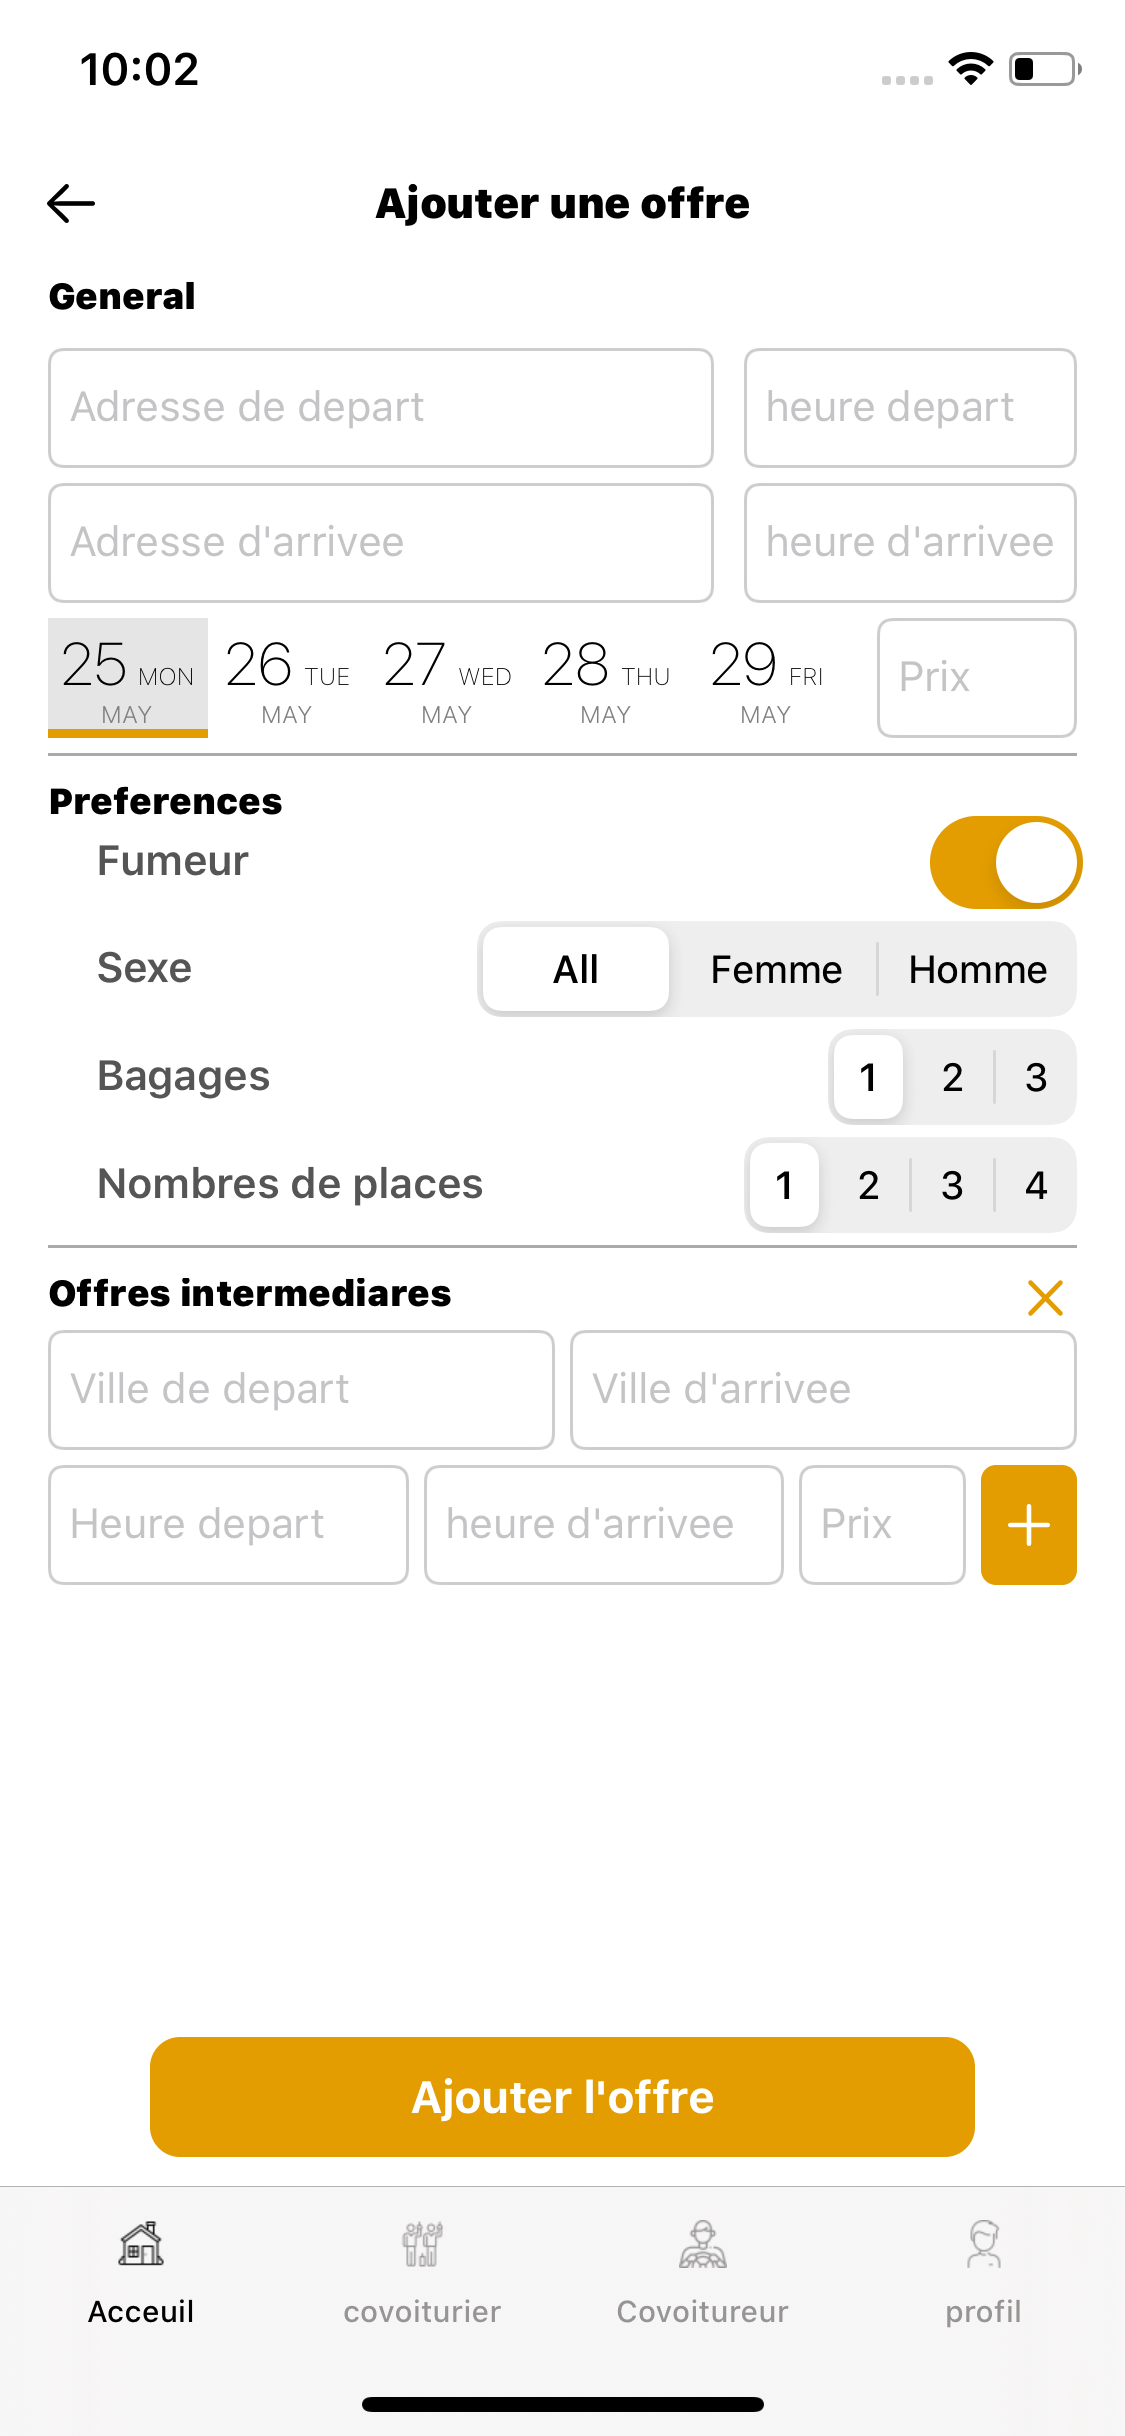
\includegraphics[width=7cm]{figs/ui2.png} }}%
    \caption{Les offres planifiés}%
    % \label{fig:example}%
\end{figure}
\clearpage
\begin{figure}%
    \centering
    \subfloat[Conducteur]{{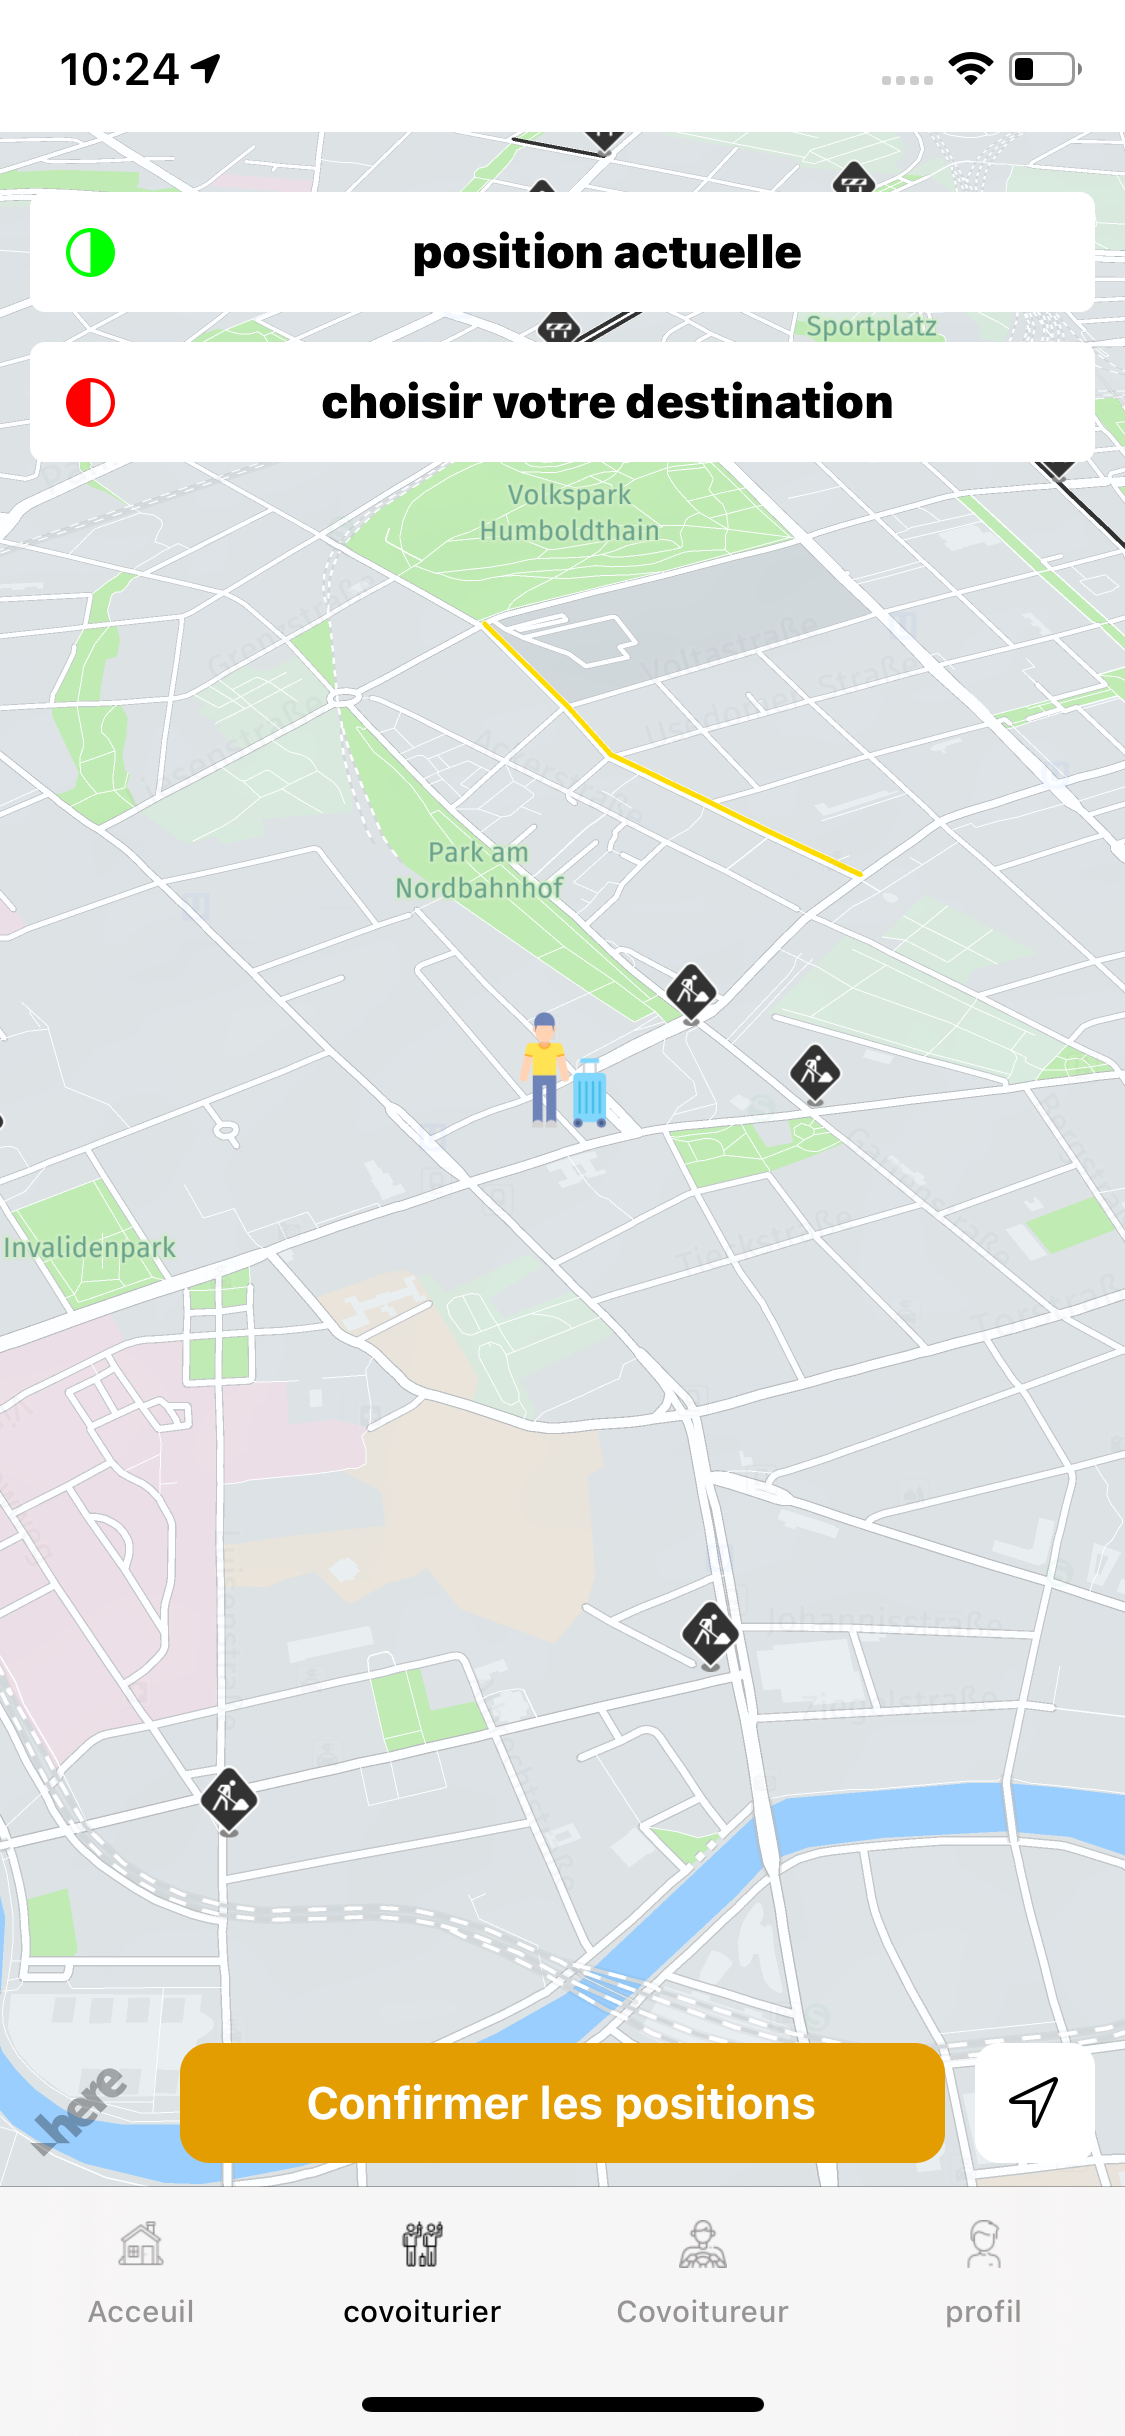
\includegraphics[width=7cm]{figs/ui3.png} }}%
    \qquad
    \subfloat[Passager]{{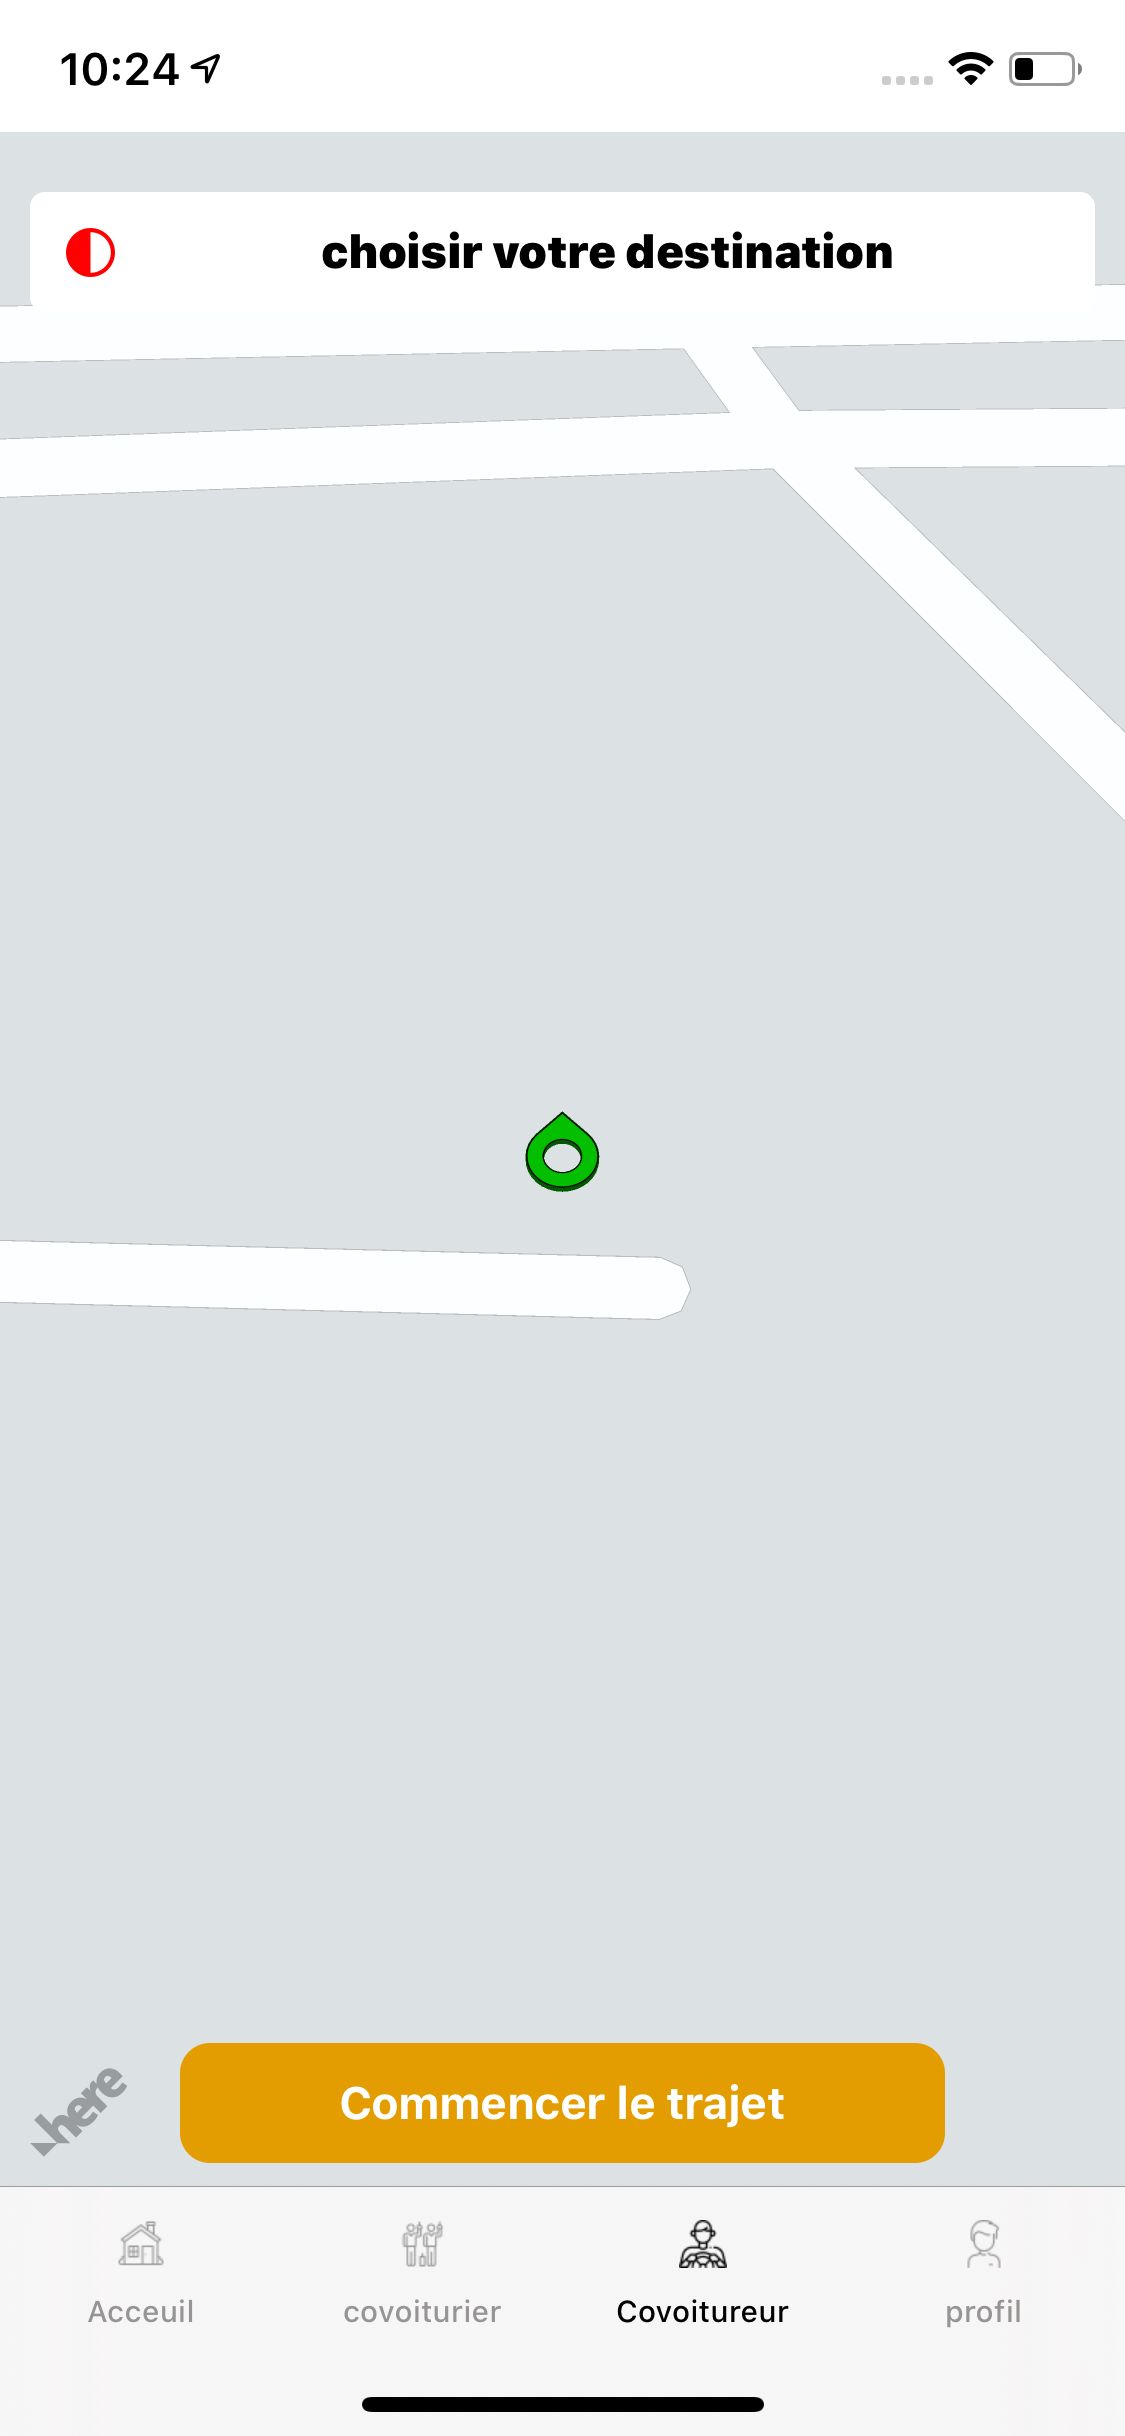
\includegraphics[width=7cm]{figs/ui4.png} }}%
    \caption{Les offres instantanés}%
    % \label{fig:example}%
\end{figure}
\clearpage
\begin{figure}%
    \centering
    \subfloat[Authentification]{{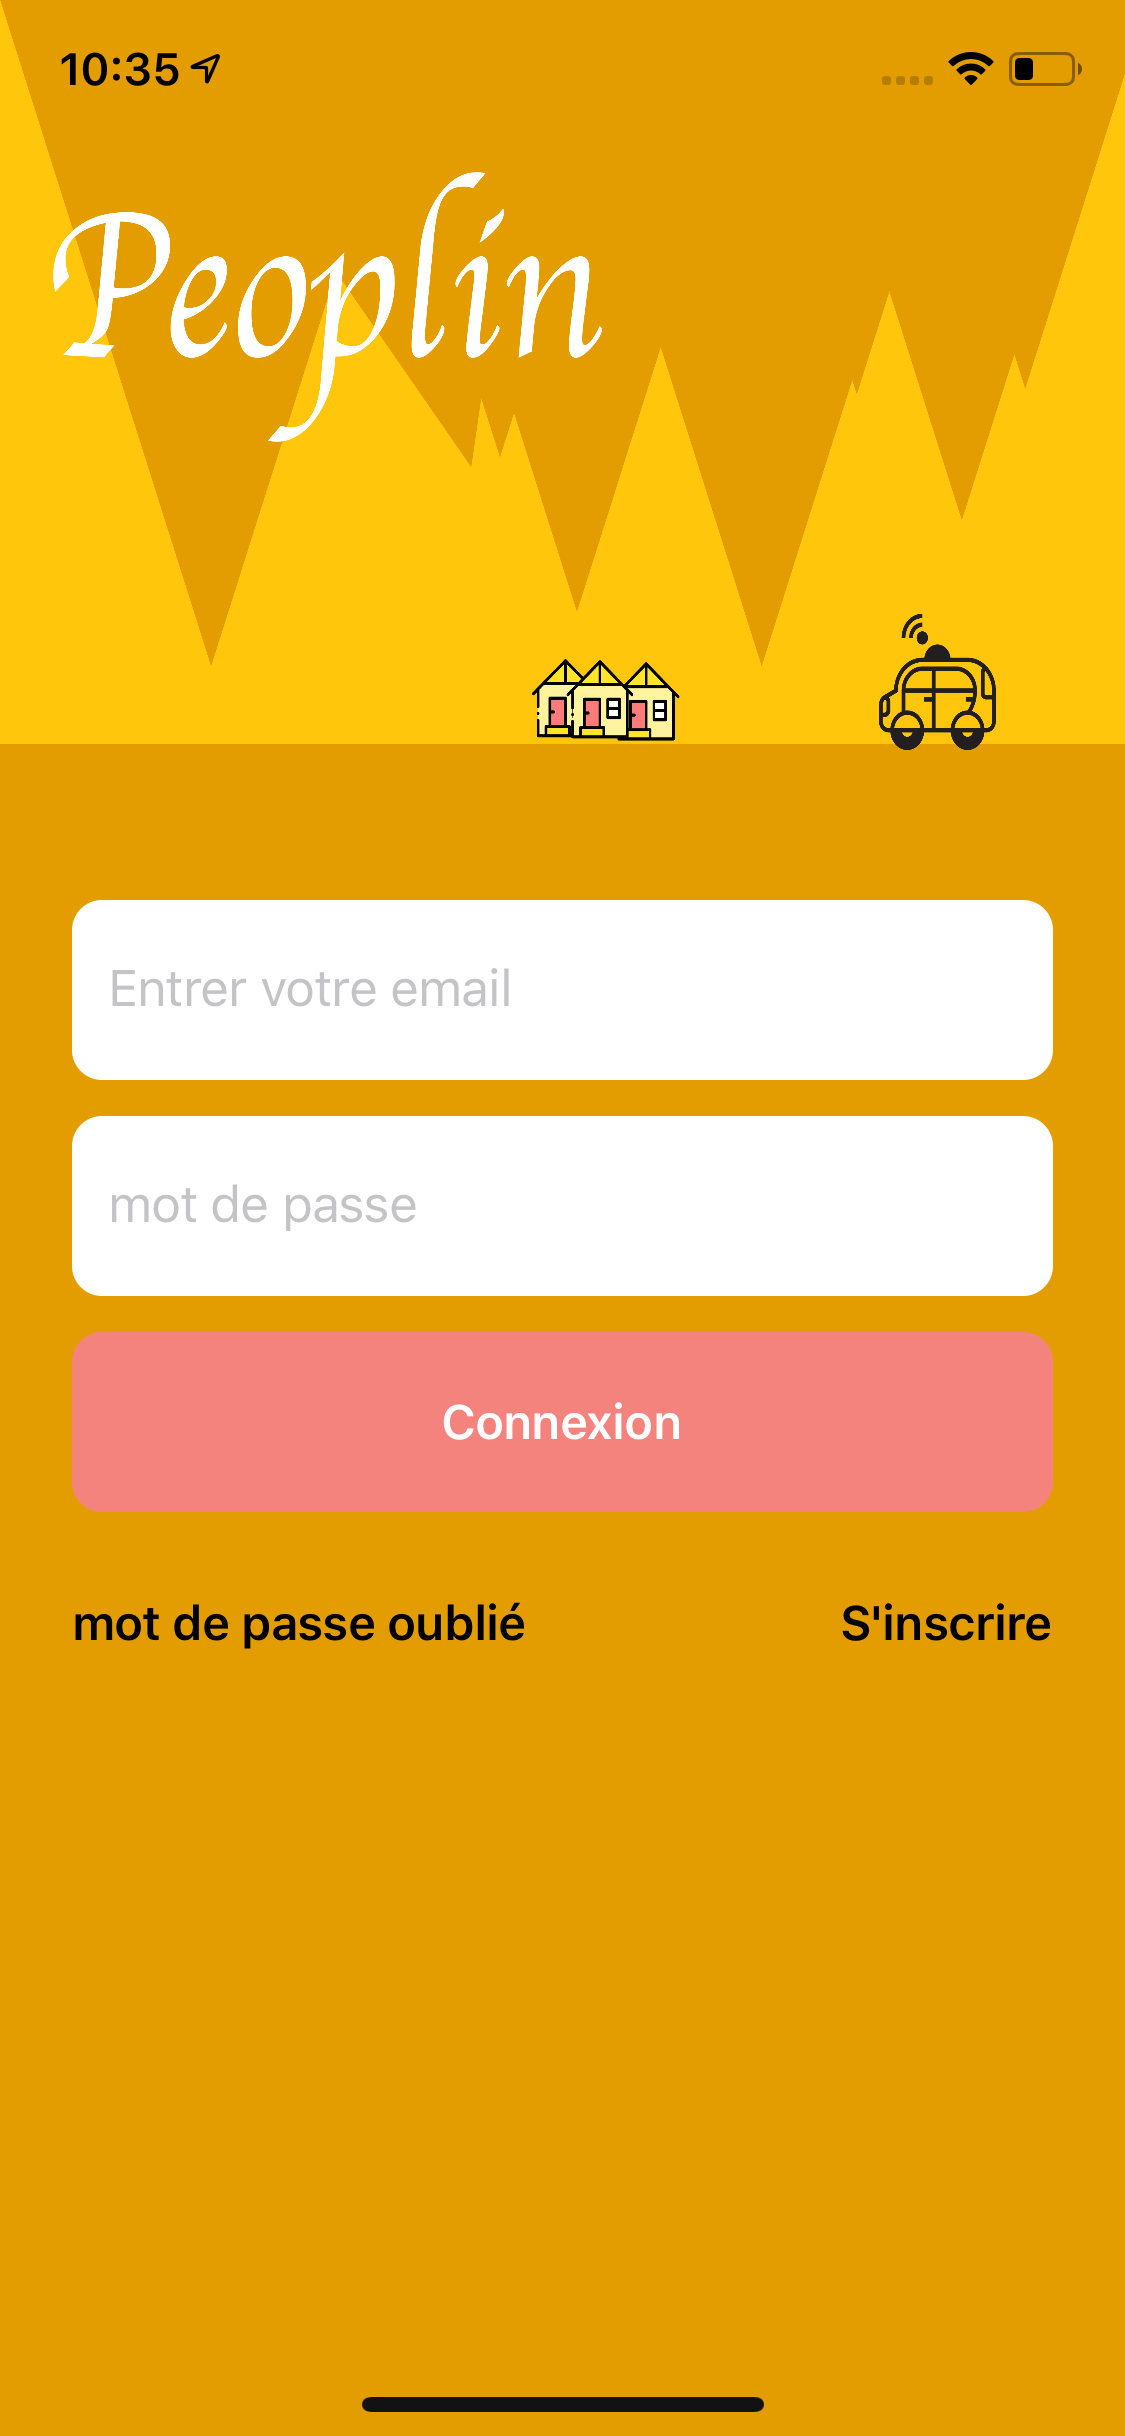
\includegraphics[width=7cm]{figs/ui6.png} }}%
    \qquad
    \subfloat[Profil]{{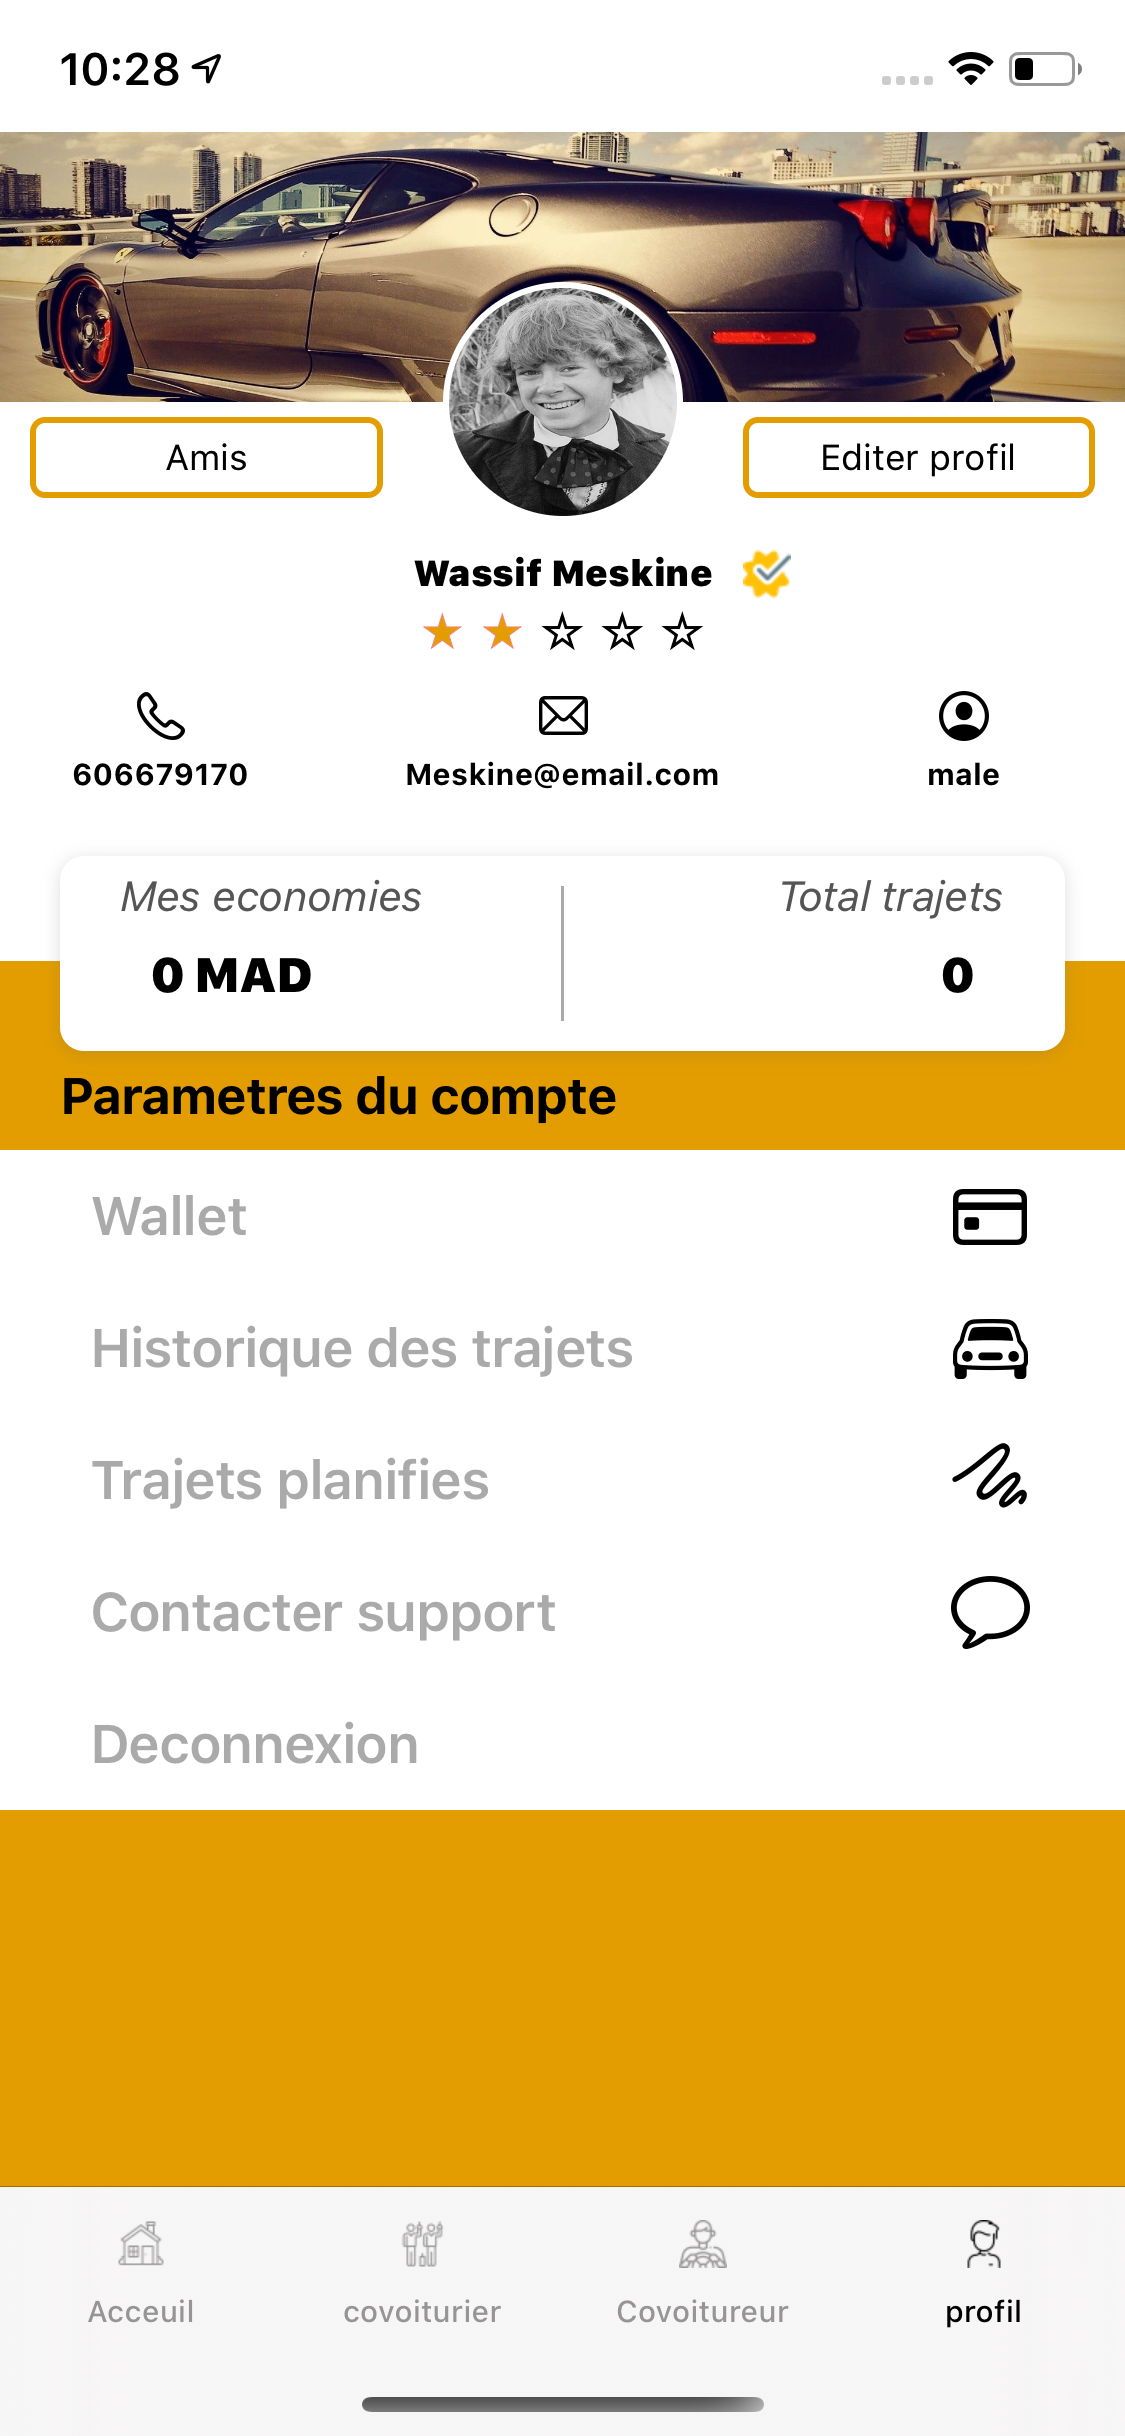
\includegraphics[width=7cm]{figs/ui5.png} }}%
    \caption{Utilisateur}%
    % \label{fig:example}%
\end{figure}
\clearpage
\begin{figure}%
    \centering
    \subfloat[Informations personnelles]{{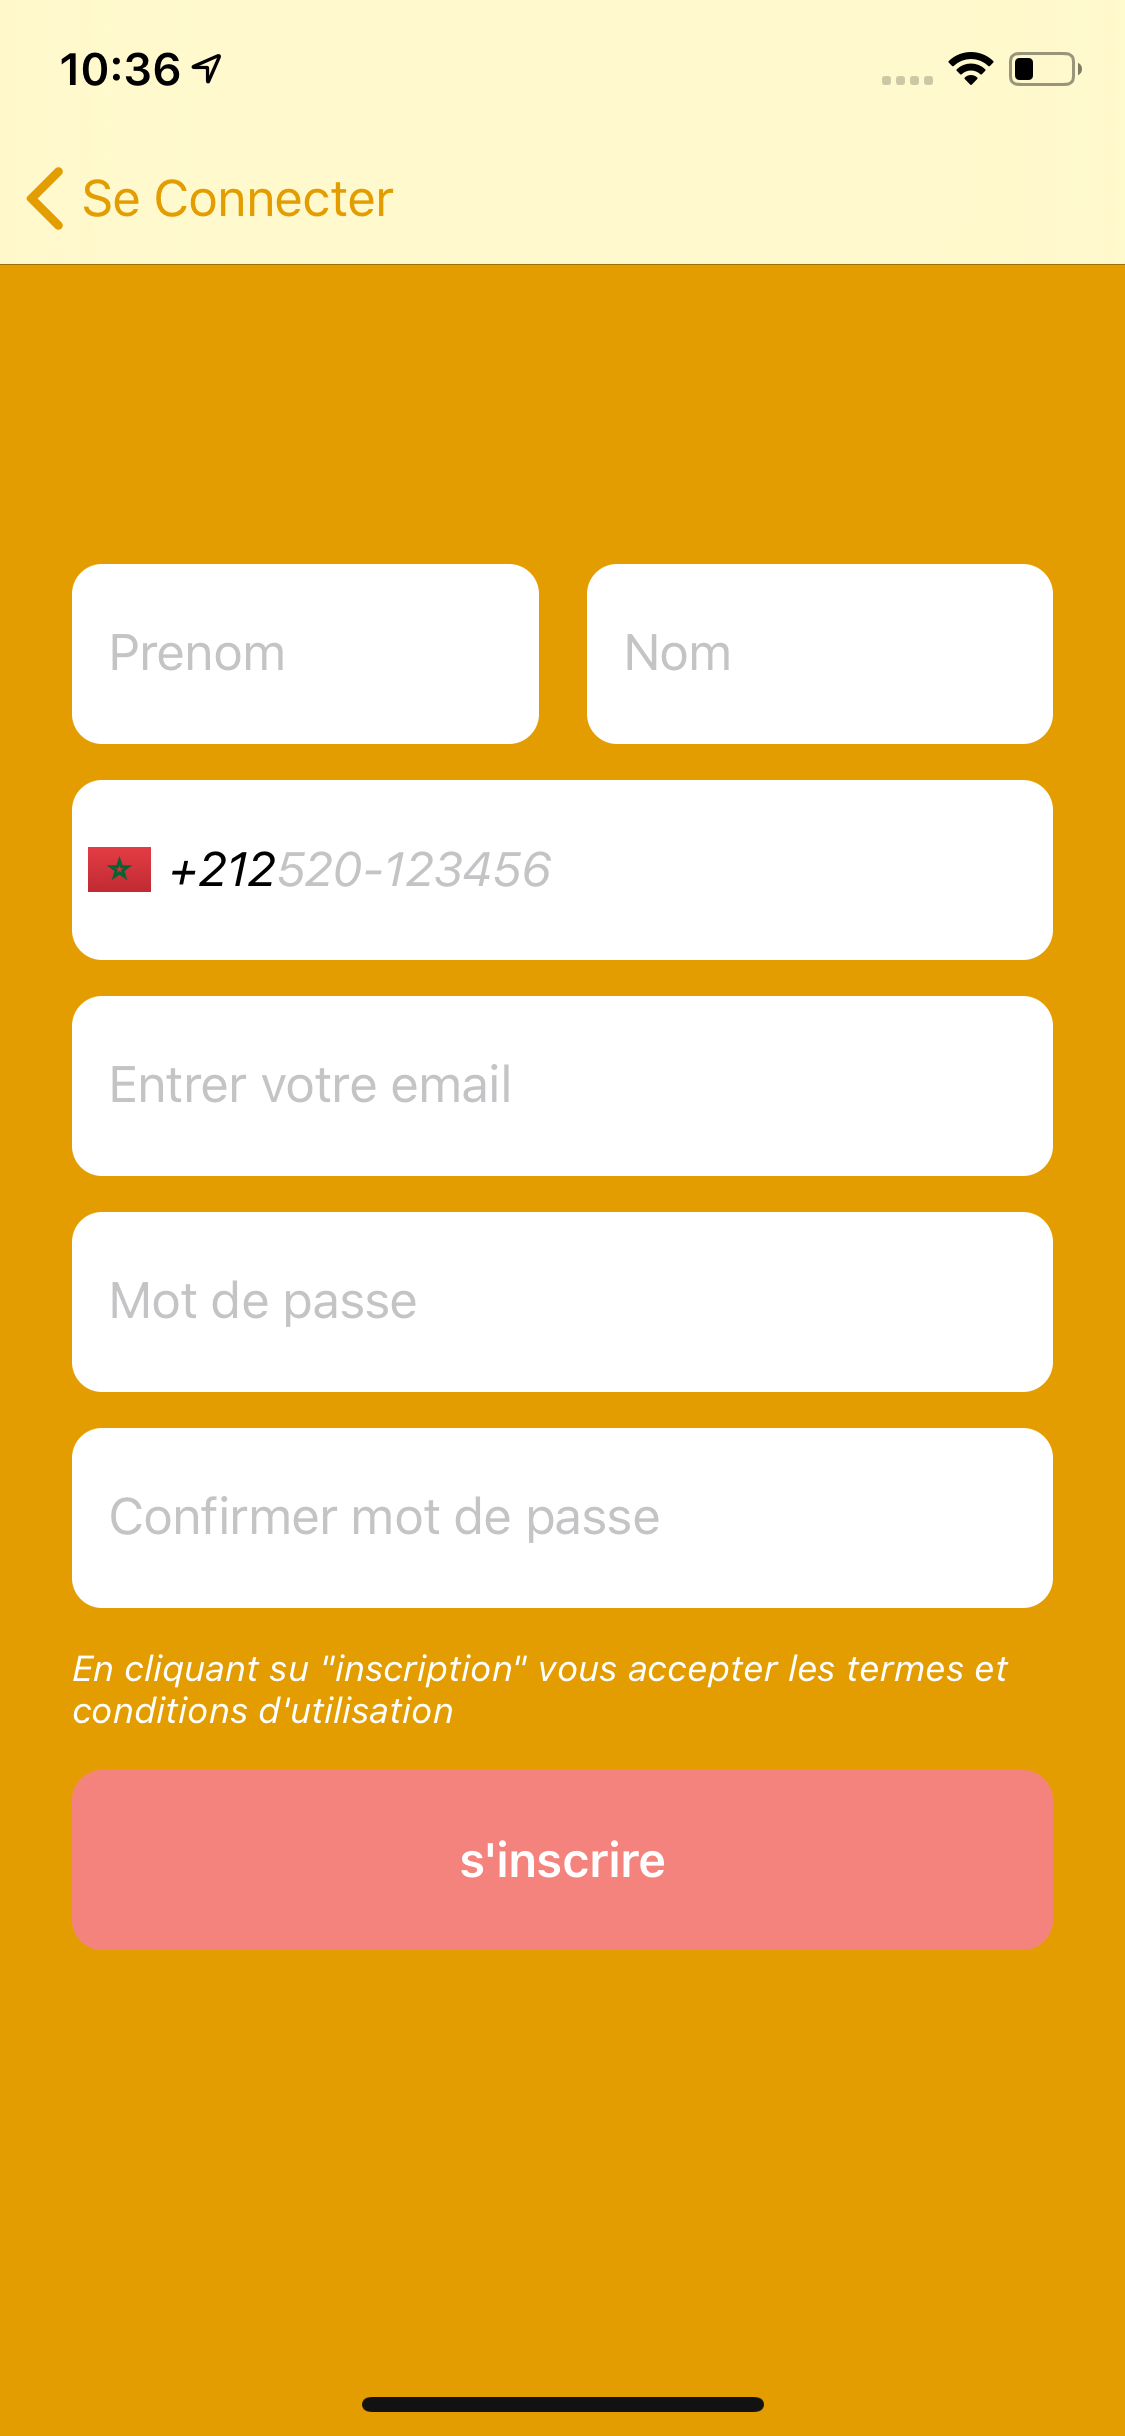
\includegraphics[width=7cm]{figs/ui7.png} }}%
    \qquad
    \subfloat[Vérification du téléphone]{{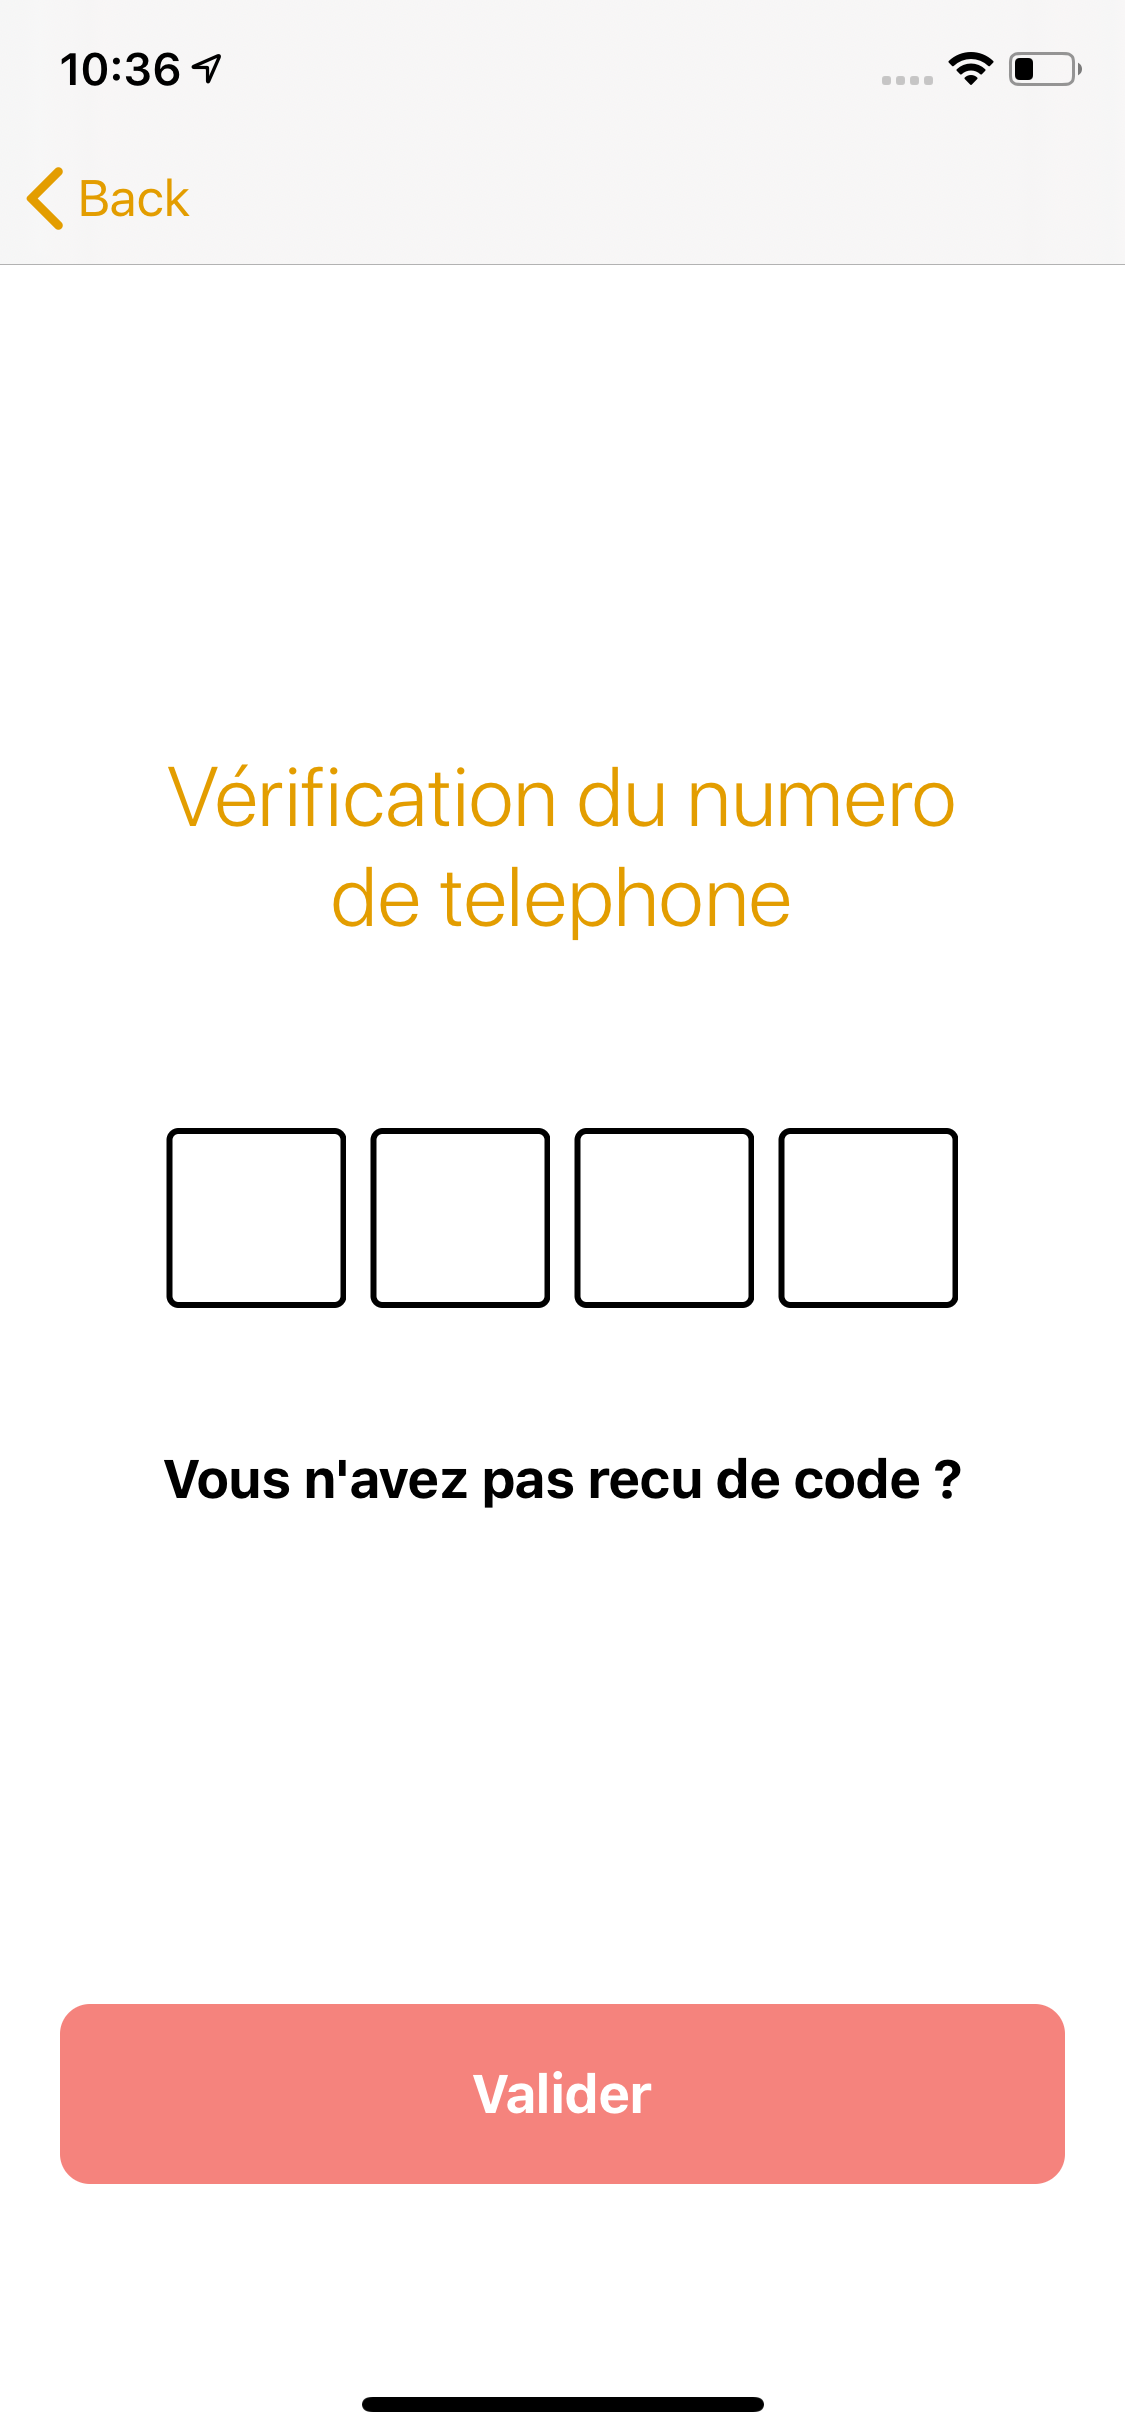
\includegraphics[width=7cm]{figs/ui8.png} }}%
    \caption{L'inscription}%
    % \label{fig:example}%
\end{figure}
\paragraph{Conclusion.} Ce troisième chapitre avait pour finalité de donner une vue d'ensemble sur l'architecture, les technologies et le choix technique.

